\begin{figure}[h]
    \centering
    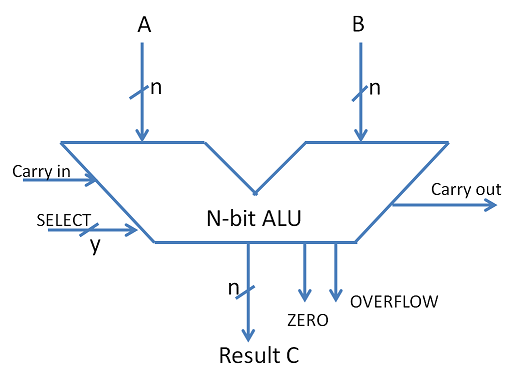
\includegraphics[scale=0.5]{ALUSYMBOLDIAG}
    \caption{Diagram Unit ALU}
    \label{fig:ALUSYMBOLDIAG}
\end{figure}

Arithmetic Logic Unit atau ALU adalah unit atau bagian CPU yang bertugas untuk
memproses kalkulasi-kalkulasi aritmatika dan operasi boolean/logika.

Menurut Ensiklopedia Brittanica, Arithmetic Logic Unit (ALU) adalah ``\dots{}unit yang
berkaitan dengan empat fungsi aritmatika dasar, yaitu pertambahan, pengurangan,
perkalian, dan pembagian, serta operasi logika tertentu seperti perbandingan antara data
dan dalam memilih prosedur untuk menjawab suatu masalah atau bedasarkan kriteria yang
sudah ditentukan diawal.\dots{}``

Secara struktural unit ini terdiri dari gerbang-gerbang logika semikonduktor
yang kemudian disusun hingga dapat memproses nilai-nilai integer biner.

Dan karena ALU hanya memproses nilai integer, terdapat juga unit yang memproses nilai-nilai
floating-point atau decimal. Unit ini disebut dengan Floating-Point Unit atau FPU.

FPU berbeda dari ALU karena, dengan ALU yang umumnya ditemui di chipset suatu CPU,
FPU lebih sering ditemui diluar chipset, dan terletak di suatu tempat lain di Motherboard.

Di diagram Gambar~\ref{fig:ALUSYMBOLDIAG} dapat disimpulkan beberapa hal, pertama suatu ALU
akan menerima dua input (A dan B di diagram), ALU juga menerima sinyal operasi apa yang akan
digunakan (SELECT di diagram), akan mengeluarkan status yang dikirim ke register yang menyimpan
status akhir suatu operasi(Carry in, Carry out, Overflow dan Zero), dan terakhir akan mengoutput
nilai dari kedua data yang telah dioperasikan.

Dan selain FPU, terdapat juga yang bernama GPU yang bertugas untuk memproses instruksi-instruksi
grafis, GPU sendiri adalah Evolusi dari cara komputer-komputer lama yang hanya bergantung
kepada CPU untuk memproses grafis. Dalam hal lokasi dimana GPU ini terletak terdapat dua variasi
yaitu GPU yang terpisah dari GPU entah itu terletak di suatu chip di motherboard atau sebagai
peripheral PCIe, dan ada juga yang terletak didalam chipset atau APU atau dengan kata lain
Integrated GPU.
